\subsection{Multimodal Fusion Analysis}
In this phase, we performed multimodal fusion by combining both facial and vocal emotional predictions assigned to each participant. This was done using a weighted fusion formula for both emotion category (A) and intensity (V), where weights were assigned per emotion based on the reliability of each modality:
 
\[
A_{fused}(e) = W_{facial}(e) \times A_{facial} + W_{vocal}(e) \times A_{vocal}
\]
\[
V_{fused}(e) = W_{facial}(e) \times V_{facial} + W_{vocal}(e) \times V_{vocal}
\]
 
Using this method, we created a new dataset with fused emotional values. These fused values were then analyzed and compared with the ground truth using different statistical methods.

\subsubsection*{Evaluation Methods}
To measure how well the fusion worked, several statistical techniques were applied.

First, we used Euclidean Distance to calculate how close the predicted emotion coordinates were to the ground truth. The formula used is:

\[
\text{euclidean\_distance}(x_1, y_1, x_2, y_2) = \sqrt{(x_1 - x_2)^2 + (y_1 - y_2)^2}
\]

Next, we applied a paired t-test to check if there was any significant improvement in the fused results compared to using facial or vocal data alone. The formula used was:

\[
t = \frac{\bar{d}}{s_d / \sqrt{n}}
\]

where $\bar{d}$ is the mean of the differences between paired observations, $s_d$ is the standard deviation of those differences, and $n$ is the number of samples.

To measure improvement, we calculated the percentage gain of the fused method over the individual modalities. The improvement formula was:

\[
\text{improvement} = \left(\frac{\text{base\_distance} - \text{fused\_distance}}{\text{base\_distance}}\right) \times 100
\]

In the implementation, it was done using:

\begin{verbatim}
facial_vs_fused = ((metrics_df['facial_distance'] - metrics_df['fused_distance']) /
                   metrics_df['facial_distance']) * 100

vocal_vs_fused = ((metrics_df['vocal_distance'] - metrics_df['fused_distance']) /
                  metrics_df['vocal_distance']) * 100
\end{verbatim}

Emotion recognition accuracy was also used as a key metric. It was calculated by dividing the number of correctly predicted emotions by the total number of samples:

\[
\text{accuracy} = \frac{\text{number\_of\_matches}}{\text{total\_number\_of\_samples}}
\]

Standard statistical functions were also used for summarizing results, such as mean and standard deviation:

\[
\bar{x} = \frac{\sum x_i}{n}, \quad s = \sqrt{\frac{\sum(x_i - \bar{x})^2}{n - 1}}
\]

These methods helped us understand how much the fusion improved the emotion recognition task and how reliable the predictions were compared to the original single-modality models.


\subsubsection*{Analysis}
The fused method consistently shows the lowest average Euclidean distance across all emotions, which means it aligns better with the ground truth compared to using facial or vocal data alone. As shown in Figure~\ref{fig:fusion-performance}, this improvement is seen across almost all emotion categories.  

\begin{figure}[H] 
    \centering
    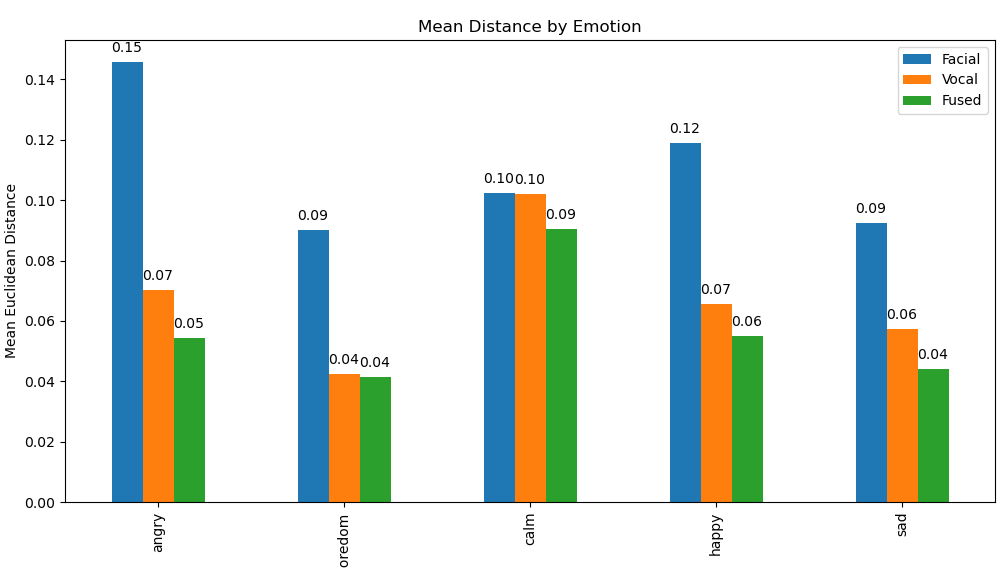
\includegraphics[width=1.1\textwidth]{img/chapter_04/fusion/emotion_performance_with_values}
    \caption{Performance comparison by Euclidean distance for each emotion}
    \label{fig:fusion-performance}
\end{figure}
 
Table~\ref{tab:mean-distances} presents the mean Euclidean distances and their standard deviations for each method:

\begin{table}[H]
  \centering
    \caption{Mean Euclidean Distances for Each Method}
    \label{tab:mean-distances}
    \begin{tabular}{l|c}
        \textbf{Method} & \textbf{Mean Distance ± Std. Dev.} \\
        \hline
        Facial & 0.1112 ± 0.0773 \\
        Vocal  & 0.0681 ± 0.0472 \\
        Fused  & 0.0577 ± 0.0481 \\
    \end{tabular}
\end{table}

The fused method’s mean distance of 0.0577 is lower than that of the vocal method (0.0681) and substantially lower than the facial method (0.1112). A lower Euclidean distance signifies predictions that are closer to the ground truth, demonstrating that the fused approach enhances accuracy by leveraging the strengths of both modalities.

To assess the statistical significance of these improvements, paired t-tests were conducted. The results are shown in Table~\ref{tab:t-test}:

\begin{table}[H]
  \centering
    \caption{T-test Results for Fused Method Comparisons}
    \label{tab:t-test}
    \begin{tabular}{l|c|c|c}
        \textbf{Comparison} & \textbf{T-Statistic} & \textbf{P-Value} & \textbf{Significant} \\
        \hline
        Facial vs Fused & 9.5129 & 0.0000 & Yes \\
        Vocal vs Fused  & 3.6117 & 0.0004 & Yes \\
    \end{tabular}
\end{table}

Both p-values are below the 0.05 threshold, confirming that the fused method’s improvements over the facial and vocal methods are statistically significant. The larger t-statistic for the facial vs. fused comparison (9.5129) compared to the vocal vs. fused comparison (3.6117) suggests a more pronounced enhancement over the facial method.


Figure~\ref{fig:heatmap-improvement} shows a visual representation of the fused method’s performance improvements over the facial and vocal methods across emotions and intensity levels. While not explored in depth here, they offer insights into specific conditions where the fused approach excels or where individual modalities may retain advantages


\begin{figure}[H]
    \centering
    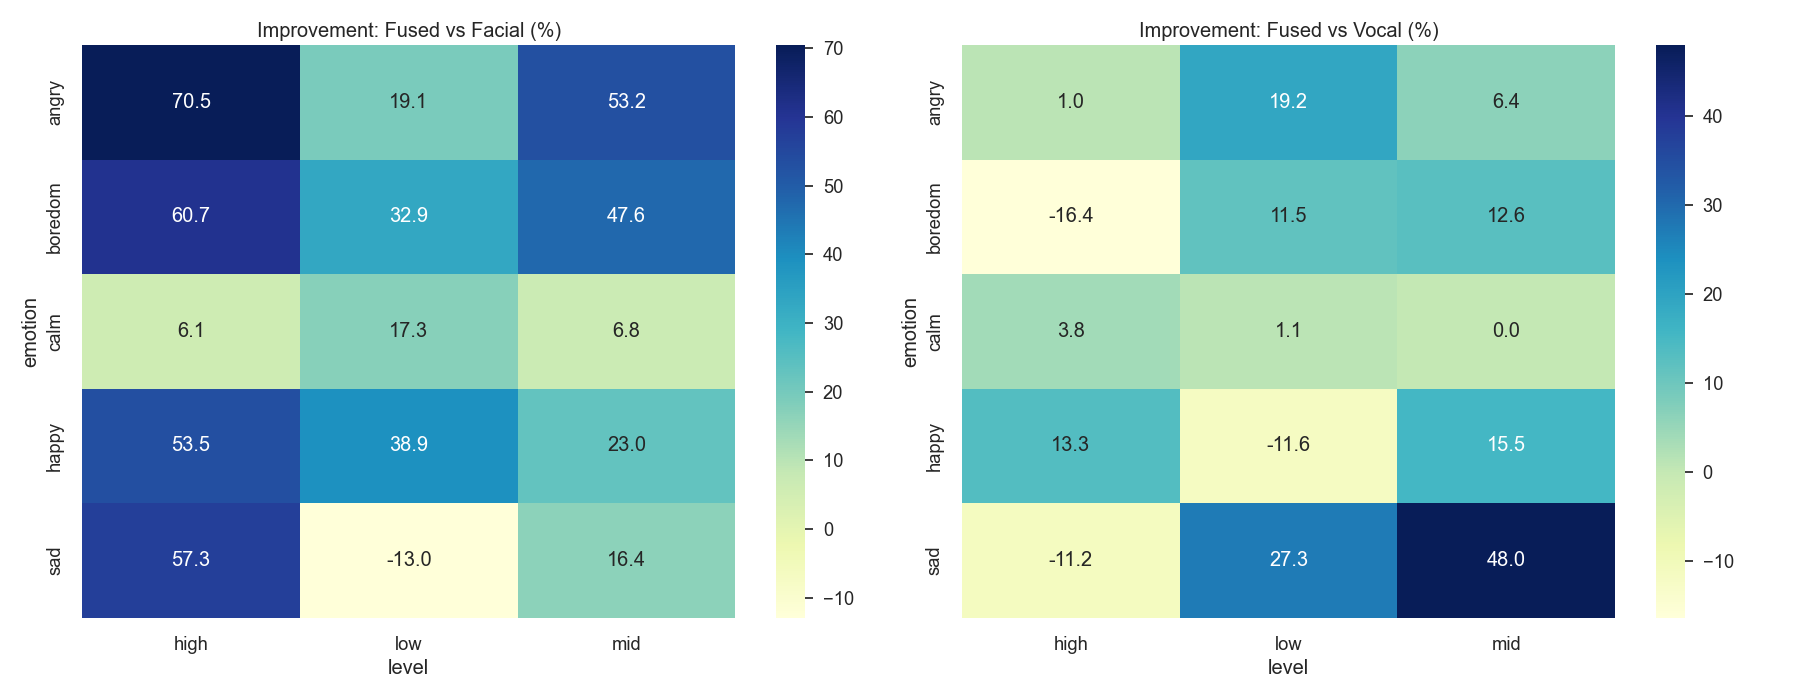
\includegraphics[width=1\textwidth]{img/chapter_04/fusion/improvement_heatmap.png}
    \caption{Improvement heatmaps: Fused vs Facial and Fused vs Vocal by Emotion and Intensity}
    \label{fig:heatmap-improvement}
\end{figure}

The fused method yields an average improvement of 33.92\% over the facial method and 6.52\% over the vocal method. This disparity reflects the vocal method’s stronger baseline performance compared to the facial method, leaving less room for improvement when fused with vocal data.
 
Emotion-wise improvements further highlight the fused method’s efficacy across different emotional categories, as shown in Figure~\ref{fig:bar-improvement}. 

The fused method consistently improves over both individual methods for all emotions. Notable gains over the facial method are observed for ``angry'' (47.58\%) and ``boredom'' (47.54\%), with the smallest improvement for ``calm'' (10.18\%). Over the vocal method, the largest improvement occurs for ``sad'' (16.27\%), while ``calm'' shows the smallest gain (1.72\%). These variations suggest that the fused method’s benefits are emotion-specific, likely influenced by the relative strengths of facial and vocal cues for each emotion.

\begin{figure}[H]
    \centering
    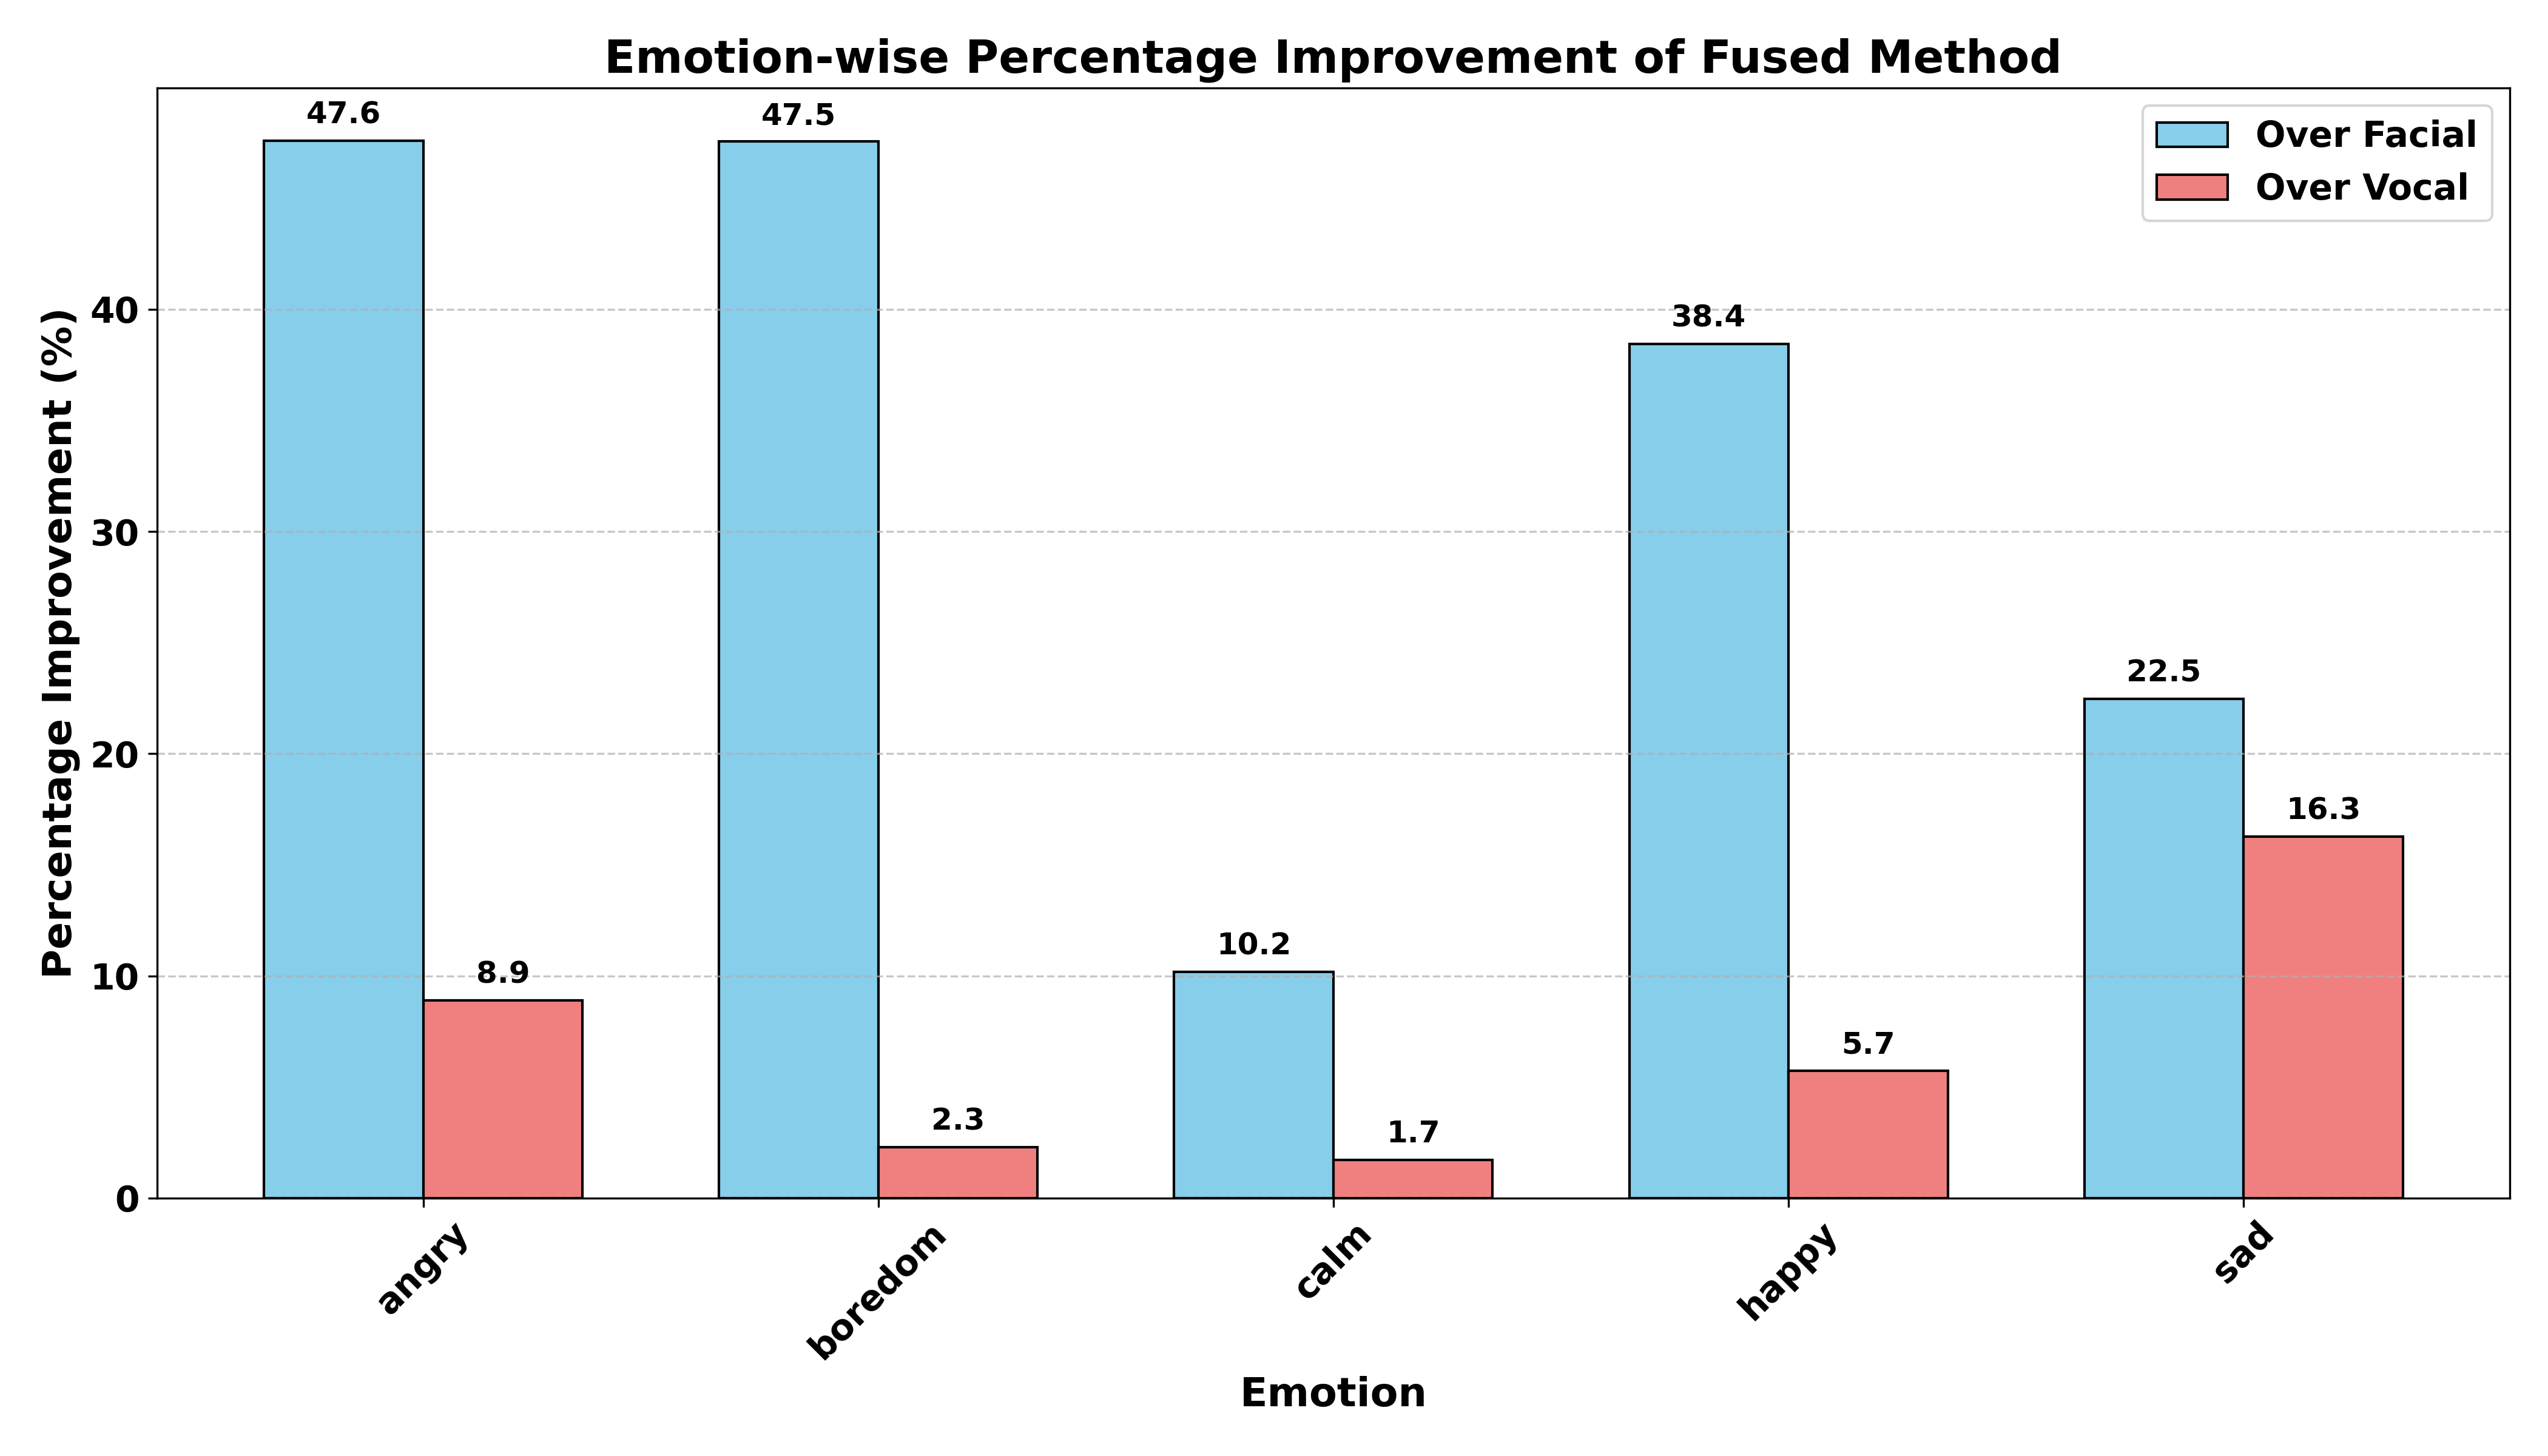
\includegraphics[width=1.05\textwidth]{img/chapter_04/fusion/statistical_improvement_by_emotion.png}
    \caption{Statistical improvement (percentage) by emotion}
    \label{fig:bar-improvement}
\end{figure}








